\section{Improving abstract propagation}
\label{sec:optim}

\begin{figure}[t]
	\centering
	\caption{\label{fig:relu-subs} ReLU split subsumption example along axis $z_1$
		(the actual lower star is collapsed to a line)}
	\begin{subfigure}{.45\textwidth}
		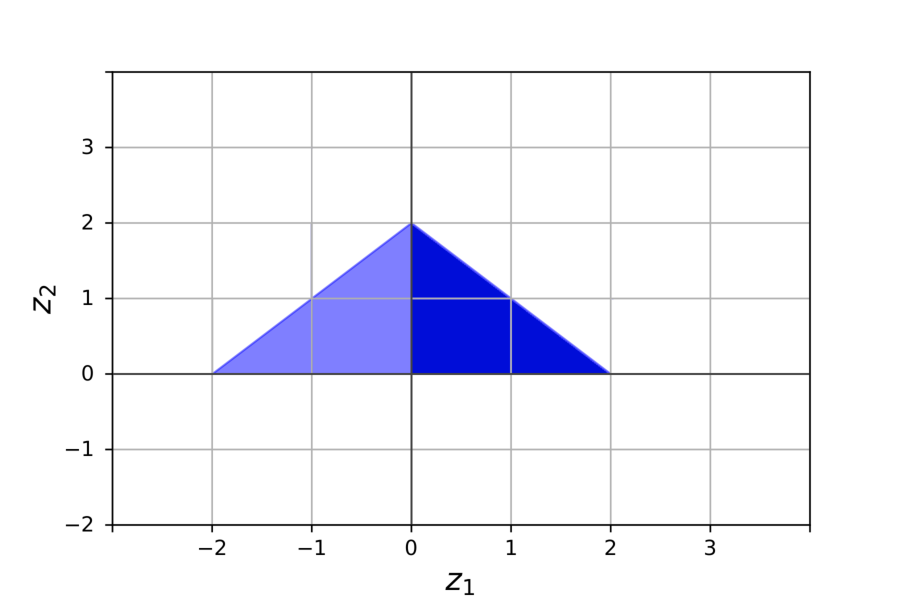
\includegraphics[width=\linewidth]{NN/Subsumed_true.pdf}
		\caption{\label{fig:relu-subs-ok}In this example the lower star can be
			subsumed by the upper one}
	\end{subfigure}
	\hspace*{\fill}
	\begin{subfigure}{.45\textwidth}
		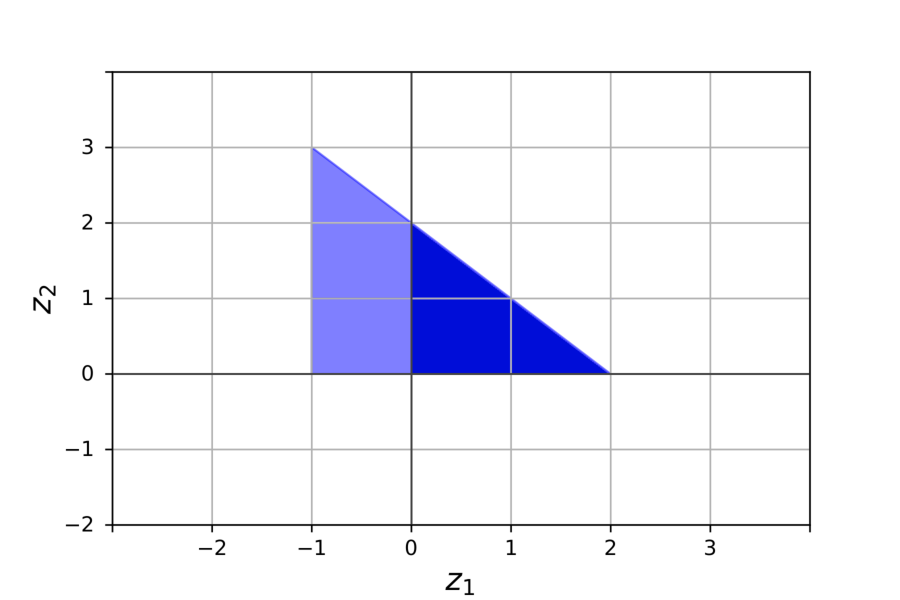
\includegraphics[width=\linewidth]{NN/Subsumed_false.pdf}
		\caption{\label{fig:relu-subs-no}In this example the lower star cannot be 
			subsumed by the upper one}
	\end{subfigure}
\end{figure}

The abstraction procedure detailed in Section~\ref{sec:abstr} allows to control the
number of stars produced during the layer propagation. Nevertheless, we can note that
the lower star in the ReLU split could be completely subsumed by the upper one depending
on the bounds along the other variables. 

Figure~\ref{fig:relu-subs} exemplifies this statement: in case~\ref{fig:relu-subs-ok}
the lower star is negligible when projected to the $z_2$ axis while in case~\ref{fig:relu-subs-no}
the projection adds information which is not present in the upper star. More formally,
we can say that if the lower star bounds along the dimension $z_2$ are lesser than the upper
star ones, then the upper star subsumes the lower on dimension $z_2$. We can generalize by
stating that for the dimension, i.e., neuron $i$ we can ignore the lower star if and only if
for all other dimensions, i.e., neurons $j = 1, ..., n$, $i \neq j$:

$$ub^j_{upp} \leq ub^j_{low} \wedge lb^j_{upp} \geq lb^j_{low}$$

The procedure is sound because the star set we obtain by the \textsc{compute\_relu} function
with the exact method in the same layer is guaranteed to contain stars with the same number
of dimensions such that the comparison is possible. Furthermore, given that ReLU does not
perform affine transformations, all stars share the same center and the dimension in the basis
matrix which is zeroed corresponds to the projection of the lower star on that dimension.

\begin{algorithm}[t]
	\caption{Star elimination algorithm}
	\label{alg:prop_v2}
	\begin{algorithmic}[1]
		\Function{get\_unique}{\emph{lower}, \emph{upper}, \emph{v}}
		\State $lower.lb_v = lower.ub_v = 0$
		\State $upper.lb_v = 0$
		\State \emph{dim\_list} = \textsc{order}(\emph{tot\_vars}, \emph{v})
		
		\For{$j$ in \emph{dim\_list}}
		\State $lb\_low_j, ub\_low_j$ = \textsc{get\_bounds}(\emph{lower}, $j$)
		\State $lb\_upp_j, ub\_upp_j$ = \textsc{get\_bounds}(\emph{upper}, $j$)
		
		\If{$ub\_upp > ub\_low$ or $lb\_upp < lb\_low$}
		\State \Return [\emph{lower, upper}]
		\EndIf
		\EndFor
		
		\State \Return [\emph{upper}]
		\EndFunction
		
		\item[]
		
		\Function{order}{\emph{num\_vars}, \emph{j}}
		\State \emph{output} = $[\:]$
		\For{$i = j + 1:num\_vars$}
		\State \textsc{append}(\emph{output}, $i$)
		\EndFor
		\For{$i = 0:j - 1$}
		\State \textsc{append}(\emph{output}, $i$)
		\EndFor
		\State \Return \emph{output}
		\EndFunction
		
		\item[]
		
		\Function{compute\_relu}{\emph{input} = $[\Gamma_1, \ldots,
			\Gamma_M]$, $j$, \emph{level}, $n$}
		
		$\ldots$
		
		\If{\emph{level} $>$ $0$}
		\State $\Theta_{low}$ = \emph{input}$[k] \wedge z[j] < 0$;
		\hspace{1ex}$\Theta_{upp}$ = \emph{input}$[k] \wedge z[j] \geq 0$
		\State $S$ = \textsc{get\_unique}($M \mbox{ * } \Theta_{low}, \Theta_{upp}, j$)
		\EndIf
		
		$\ldots$
		
		\EndFunction
	\end{algorithmic}
\end{algorithm}

Algorithm~\ref{alg:prop_v2} details the procedure for checking the elimination of
the lower star. In order to contain the number of LPs to solve, since each dimension
is processed subsequently, we start checking the dimensions following the one 
alongside which the ReLU split occurred: in this way, even if the check fails, the
LP does not add extra computational time as it is used for the next neuron. This
is obtained by function \textsc{order} in line $4$. 
After ordering the dimensions, we perform the subsumption check for each one of them;
whenever this check fails, both the lower and the upper star are returned without
spending further time checking other dimensions (line $9$). Only if the check is 
successful for every dimension, the function returns the upper star only (line $10$).
This modification is highlighted in the fragment of \textsc{compute\_relu} in lines
$18 - 22$. The cost for the extra LPs paid when the upper star subsumes the lower is 
balanced by the reduction of the number of stars that are propagated, whereas if the
subsumption check fails soon enough, no extra LPs are computed since the bounds are
used in the next neuron computation. The worst case scenario is a check that takes
almost all the dimensions to finally fail, which leads eventually to a major overhead.